\chapter{Konttien orkestrointi\label{orchestration}}

Konttiteknologiaa käytetään kasvavissa määrissä monilla ohjelmistotuotannon osa alueilla.
Konttiteknologia mahdollistaa fyysisen palvelimen tai ohjelmistökehittäjän tietokoneen suoritusympäristöstä eroavan vakaan ja rajattomasti toistettavan ympäristön \cite{Watada19}.
Konttiteknologian kasvava käyttö on luonut tarpeen hallinnoida suuria määriä kontteja samanaikaisesti.
Tähän tarpeeseen pyrkivät vastaamaan erilaiset konttiorkestraatioalustat.

Konttiorkestraatioalustat hallinnoivat suuria määriä kontteja jaetussa klusterissa.
Orkestraatioalustat, kuten Kubernetes, mahdollistavat muun muassa palveluiden replikoinnin, tehokkaan julkaisuketjun, kontitettujen palveluiden monitoroinnin ja virhetiloista toipumisen \cite{Khan17}.

\section{Kontti}

Kontti on karsittu ympäristö, joka koostuu palvelusta ja sen tarvitsemista riippuvuuksista.
Kontti tarjoaa vakaan ja suljetun ympäristön palvelun suorittamiselle \cite{Watada19}.
Kontti on riippumaton fyysisestä palvelimesta ja sen ulkopuolisestä ympäristöstä, joka mahdollistaa saman kontin toistamisen muilla palvelimilla ja alustoilla \cite{Kang16}.

Virtuaalikonejulkaisuista poiketen useampi kontti voi jakaa resursseja ja näin ollen esimerkiksi käyttöjärjestelmän ydintä ei tarvitse säilöä erikseen jokaiseen konttiin.
Tämän seurauksena kontit ovat kokonsa ja käynnistysnopeudensa suhteen virtualisointia tehokkaampi ratkaisu \cite{Dua14}.
Kuva~\ref{fig:container} esittää resurssien jaon eri julkaisuratkaisuilla.

Yleisesti käytettyjä konttiteknologiapalveluita ovat Docker ja Podman \cite{Abraham20, Bernstein14}.
Docker on suosittu ratkaisu, mutta vaatii toimiakseen aina käynnissä olevan palveluprosessin ja root-oikeudet palvelua suorittavaan käyttöjärjestelmään \cite{Abraham20}.
Nämä tekniset ongelmat ratkaisee esimerkiksi Podman, joka toimii ilman erillistä palveluprosessia ja root-oikeuksia \cite{Gantikow20}.

\pagebreak % remove later if possible

\begin{figure}[ht]
\begin{center}
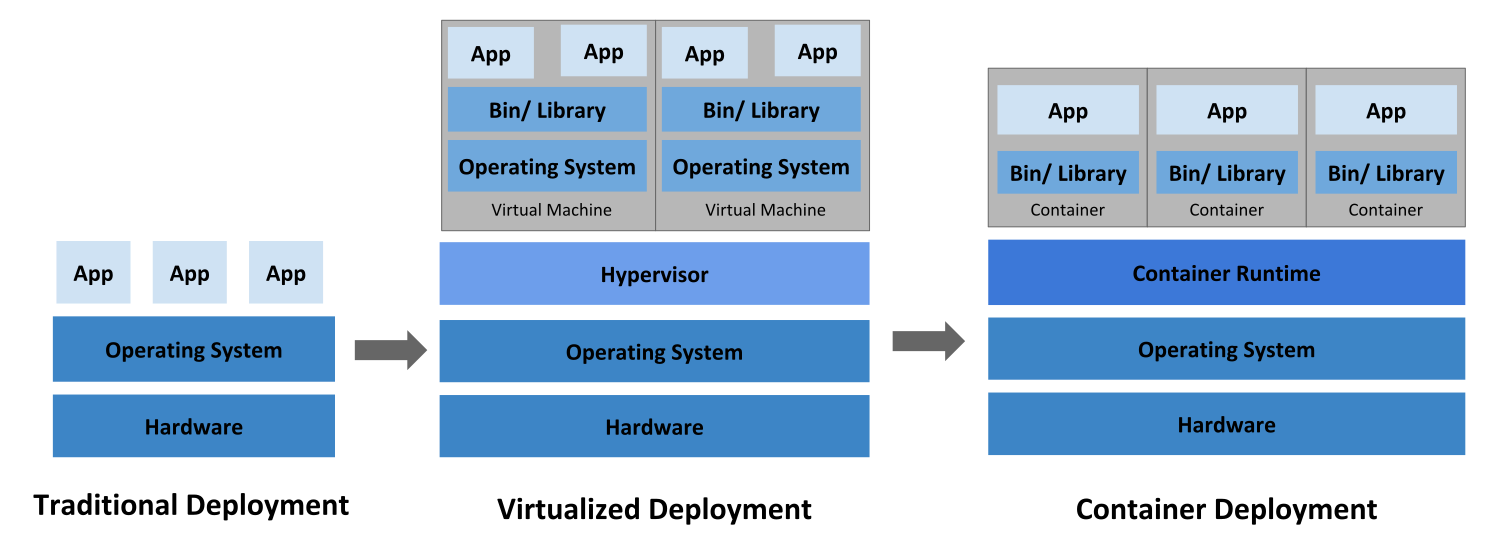
\includegraphics[width=0.9\textwidth]{figures/container_evolution.png}
\caption{Sovelluksen omat ja jaetut resurssit eri julkaisutavoilla.\cite{Kubernetes23}\label{fig:container}}
\end{center}
\end{figure}

\section{Konttiorkestraatioalustat}

% Rewrite later

Erityisesti mikropalvelupohjaiset järjestelmät saattavat koostu useista sadoista konteista.
Myös muun muassa saman palvelun replikaatio ja alueellinen hajauttaminen luovat tarpeen hallinnoida suuria määriä kontteja \cite{Khan17}.
Konttiorkestraatioalustat ovat järjestelmiä, joiden tehtävä on mahdollistaa suurien konttimäärien hallinnointi.
Orkestraatioalustat muun muassa hallinnoivat konttien resurssien käyttöä, mahdollistavat konttien monitoroinnin ja huolehtivat konttien virhetilanteista toipumisesta \cite{Zhou21}.

Kubernetes on laajalti käytetty konttiorkestraatioratkaisu. Se on nykyisistä ratkaisuista suorituskyvyltään tehokkain ja myös toiminnallisuuksiltaan kattavin \cite{Jawarneh19}. Muita ratkaisuja ovat muun muassa Docker Swarm ja Amazon Elastic Container Service \cite{Khan17}. Tässä tutkielmassa konttien orkestrointia käsitellään pääasiassa Kuberneteksen kautta.

% write something about kubernetes

Kubernetes on alkujaan Google kehittämä ja nykyään Linux Foundationin alla toimivan Cloud Native Foundationin hallinnoima avoimen lähdekoodin projekti \cite{Burns22}.

\section{Konttien orkestrointi ja DevOps-toimintamalli}
